\makeatletter
\def\input@path{{template/}}
\makeatother

\documentclass[]{beamer}

\usepackage[english]{babel}
\usepackage[utf8]{inputenc}
\usepackage[T1]{fontenc}
\usepackage{csquotes}
\usepackage{expl3,biblatex}
\addbibresource{example.bib}
\usepackage{booktabs}
\usetheme[workplace=fi]{MU}
\usepackage{graphicx}
\usepackage{amsmath}
\DeclareMathOperator*{\argmax}{argmax}
\DeclareMathOperator*{\argmin}{argmin}

\title[Word Translation Without Parallel Data]{Word Translation Without Parallel Data (2018)}
\subtitle[]{A. Conneau, G. Lample, M. Ranzato, L. Denoyer, H. Jégou}
\author[ ]{Poster by: A. Puigdemont Monllor, J. Čieško\texorpdfstring{\\}{, }}
\institute[FI MU]{Faculty of Informatics, Masaryk University}
\date{November 11, 2024}
\subject{PA164: Machine Learning and NLP}
\keywords{Machine Learning, NLP, Word Translation}

\begin{document}

\begin{frame}[plain]
\maketitle
\end{frame}

\section[]{Model Overview}
\begin{frame}{Model Overview}
    \small
    \textbf{Embedding Spaces and Translation Mapping}
    \begin{itemize}
        \item We assume two sets of embeddings $X$ (source) and $Y$ (target), trained independently on monolingual data.
        \item Objective: Learn a linear mapping matrix $W$ such that translations are close in a shared embedding space. This is achieved by minimizing:
        \begin{equation}
\begin{split}
            W^* = \argmin_{W \in M_d(\mathbb{R})} || W X - Y ||_F \\
	|| A ||_F = \sqrt{\sum_{i=1}^m \sum_{j=1}^n |a_{ij}|^2}	
	\end{split}
        \end{equation}
        \item Translation of a source word $s$ is computed by finding the target $t$ that maximizes the cosine similarity:
        \begin{equation}
            t = \argmax_{t} \cos(W x_s, y_t)
        \end{equation}
    \item The approach draws on prior work (Mikolov et al., 2013) that demonstrated successful alignment with a linear mapping.
    
	\end{itemize}
\end{frame}
\begin{frame}{Method Illustration}
    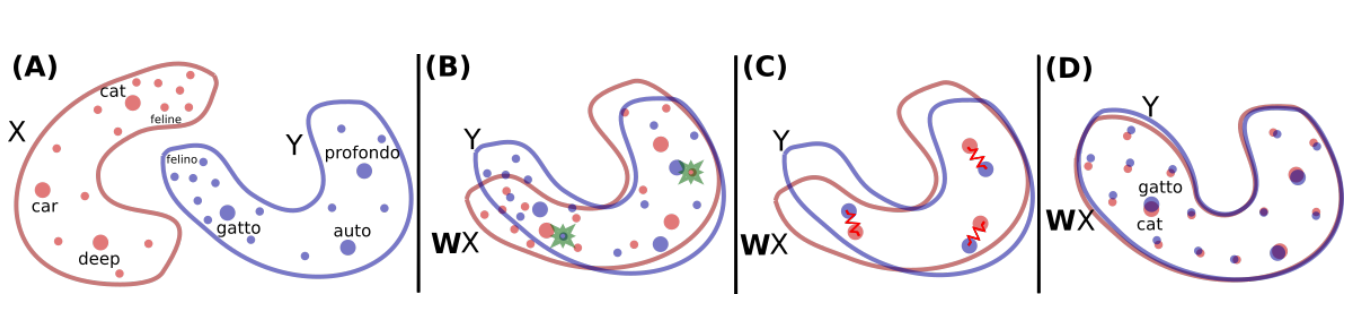
\includegraphics[width=1.0\linewidth]{figures/figure1.png}
\small
\textit{(A) The embeddings of English (red, $X$) and Italian (blue, $Y$) words are shown, where dot size indicates word frequency. (B) Adversarial learning is used to align $X$ and $Y$ with a rotation matrix $W$, tested using randomly selected words. (C) The mapping $W$ is refined through Procrustes, using frequent words as anchor points to minimize an energy function. (D) Translation uses $W$ and CSLS, which adjusts distances in dense regions to reduce "hub" effects, ensuring better word vector alignment.}
\end{frame}

\begin{frame}{Adversarial Training}
    \small
    \textbf{Domain-Adversarial Approach}
    \begin{itemize}
        \item We use a domain-adversarial approach to learn the mapping $W$ without relying on cross-lingual supervision.
        \item Let $X = \{x_1, \ldots, x_n\}$ and $Y = \{y_1, \ldots, y_m\}$ be two sets of word embeddings from a source and a target language, respectively.
        \item A \textbf{discriminator} is trained to distinguish between the transformed embeddings $WX$ and the target embeddings $Y$. This forms a two-player game:
        \begin{itemize}
            \item The discriminator aims to maximize its ability to identify the origin of an embedding.
            \item The mapping $W$ is optimized to minimize the discriminator's predictive accuracy by making $WX$ and $Y$ as similar as possible.
        \end{itemize}
        \item Discriminator's objective:
        \scriptsize
        \begin{equation}
            L_D(\theta_D | W) = - \frac{1}{n} \sum_{i=1}^n \log P_{\theta_D}(\text{source} = 1 | W x_i) - \frac{1}{m} \sum_{i=1}^m \log P_{\theta_D}(\text{source} = 0 | y_i)
        \end{equation}
	\small
        %\item This method aligns with previous work (Ganin et al., 2016) that focuses on learning representations that are invariant to the input domain (where a domain is represented by a language).
    \end{itemize}
\end{frame}

\begin{frame}{Mapping Objective}
    \small
    \textbf{Training the Mapping}
    \begin{itemize}
        \item The mapping matrix $W$ is optimized to make it difficult for the discriminator to accurately predict the origins of the embeddings:
        \scriptsize 
        \begin{equation}
            L_W(W | \theta_D) = - \frac{1}{n} \sum_{i=1}^n \log P_{\theta_D}(\text{source} = 0 | W x_i) - \frac{1}{m} \sum_{i=1}^m \log P_{\theta_D}(\text{source} = 1 | y_i)
        \end{equation}
	\small
        \item This training process involves \textbf{stochastic gradient updates}, alternating between training the discriminator and updating $W$. 
        \item The goal is to ensure that $WX$ and $Y$ become indistinguishable, thus learning a more robust mapping.
        \item This process follows the standard adversarial training protocols established by Goodfellow et al. (2014), where models are trained in opposition to each other to improve performance.
    \end{itemize}
\end{frame}

\begin{frame}{Refinement Procedure}
    \small
    \textbf{Refining the Mapping with Procrustes}
    \begin{itemize}
        \item The initial mapping $W$ from adversarial training performs well but struggles with rare words, which often have less reliable embeddings.
        \item Frequent words serve as reliable anchors for refinement to enhance alignment quality.
        \item We aim to minimize the difference between aligned embeddings:
        \begin{equation}
            W^* = \argmin_{W \in O_d(\mathbb{R})} || W X - Y ||_F
        \end{equation}
        \item A synthetic vocabulary is formed using mutual nearest neighbors among frequent words for a high-quality dictionary.
        \item The Procrustes method is applied iteratively for further refinement, but improvements beyond the first iteration are typically small, often below 1\%.
    \end{itemize}
\end{frame}

%\section[CSLS]{Cross-Domain Similarity Local Scaling (CSLS)}

\begin{frame}{Cross-Domain Similarity Local Scaling (CSLS)}
    \small
    \textbf{Improving Nearest Neighbor Matching}
    \begin{itemize}
        \item CSLS enhances the reliability of matching pairs across languages by adjusting the similarity metric.
        \item The similarity measure is defined as:
        \begin{equation}
            CSLS(W x_s, y_t) = 2 \cos(W x_s, y_t) - r_T(W x_s) - r_S(y_t)
        \end{equation}
        \item Where:
	\scriptsize
        \begin{equation}
            r_T(W x_s) = \frac{1}{K} \sum_{y_t \in N_T(W x_s)} \cos(W x_s, y_t) \quad \text{(mean similarity to target neighbors)}
	\end{equation}
	\begin{equation}
            r_S(y_t) = \frac{1}{K} \sum_{x_s \in N_S(y_t)} \cos(x_s, y_t) \quad \text{(mean similarity to source neighbors)}
        \end{equation}
	\small
        \item CSLS effectively addresses the hubness problem, where some words (hubs) serve as nearest neighbors for many others, leading to inaccuracies in translation.
        \item This method improves accuracy by scaling similarity based on the density of neighboring words, enhancing translation quality.
    \end{itemize}
\end{frame}





%\section{\bibname}
%\begin{frame}[t, allowframebreaks]{\bibname}
%\printbibliography[heading=none]
%\end{frame}

\begin{frame}[plain]
\vfill
\centerline{Thank You for Your Attention!}
\vfill
\end{frame}


\end{document}
